\documentclass[tikz,border=3pt]{standalone}
\usepackage[utf8]{inputenc}
\usepackage[T1]{fontenc}
\usepackage{lmodern}
\renewcommand{\familydefault}{\sfdefault}
\usepackage{sansmath}\sansmath
\usepackage{chemfig}
\usepackage{pgfplots}\pgfplotsset{compat=1.18,/pgf/number format/use comma,/pgf/number format/1000 sep={.}}
\usetikzlibrary{arrows.meta,calc,positioning,decorations.pathmorphing,patterns}
% paleta del sitio
\definecolor{nar}{HTML}{E8680C}\definecolor{narc}{HTML}{FFB35C}\definecolor{hielo}{HTML}{FFF3E8}
\definecolor{tinta}{HTML}{1D1D1F}\definecolor{gris}{HTML}{6E6E73}\definecolor{lila}{HTML}{7C5CF0}
\definecolor{azul}{HTML}{2F6FD6}\definecolor{menta}{HTML}{17A673}\definecolor{coral}{HTML}{E8342A}
\begin{document}
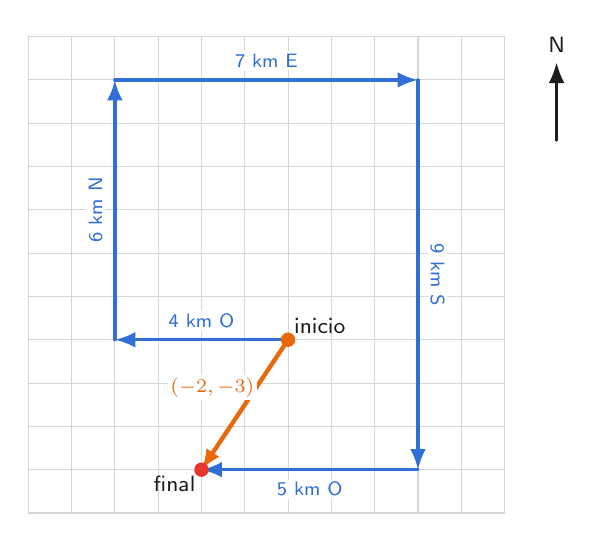
\begin{tikzpicture}[font=\small,x=0.55cm,y=0.55cm,line cap=round,line join=round,step={(1,1)}]
\draw[gris!28,thin] (-6,-4) grid (5,7);
\draw[-{Latex[length=2.6mm,width=2mm]},very thick,azul] (0,0)--(-4,0);
\draw[-{Latex[length=2.6mm,width=2mm]},very thick,azul] (-4,0)--(-4,6);
\draw[-{Latex[length=2.6mm,width=2mm]},very thick,azul] (-4,6)--(3,6);
\draw[-{Latex[length=2.6mm,width=2mm]},very thick,azul] (3,6)--(3,-3);
\draw[-{Latex[length=2.6mm,width=2mm]},very thick,azul] (3,-3)--(-2,-3);
\node[font=\scriptsize,text=azul,fill=white,inner sep=1pt] at (-2,0.45) {4 km O};
\node[font=\scriptsize,text=azul,fill=white,inner sep=1pt,rotate=90] at (-4.45,3) {6 km N};
\node[font=\scriptsize,text=azul,fill=white,inner sep=1pt] at (-0.5,6.45) {7 km E};
\node[font=\scriptsize,text=azul,fill=white,inner sep=1pt,rotate=-90] at (3.45,1.5) {9 km S};
\node[font=\scriptsize,text=azul,fill=white,inner sep=1pt] at (0.5,-3.45) {5 km O};
\draw[-{Latex[length=2.6mm,width=2mm]},ultra thick,nar] (0,0)--(-2,-3);
\fill[nar] (0,0) circle (2.6pt) node[above right,font=\footnotesize,text=tinta,inner sep=2pt] {inicio};
\fill[coral] (-2,-3) circle (2.6pt) node[below left,font=\footnotesize,text=tinta,inner sep=2pt] {final};
\node[font=\scriptsize,text=nar,fill=white,inner sep=1pt] at (-1.75,-1.1) {$(-2, -3)$};
\draw[-{Latex[length=2.6mm,width=2mm]},thick,tinta] (6.2,4.6)--(6.2,6.4) node[above,font=\footnotesize] {N};
\end{tikzpicture}
\end{document}
